\section{Image Segmentation}

\begin{frame}{Trainingseingaben}
    \begin{figure}
        \centering
        \begin{subfigure}{0.495\textwidth}
            \centering
            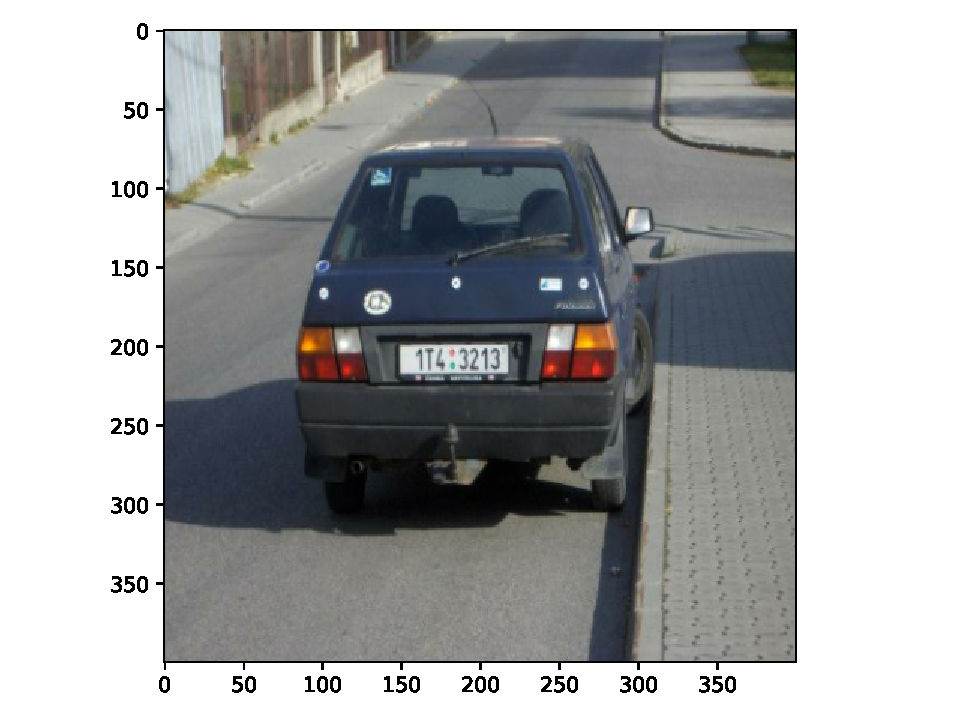
\includegraphics[width=\textwidth]{img/model_demo_1}
            \caption{Eingabe}
        \end{subfigure}
        \begin{subfigure}{0.495\textwidth}
            \centering
            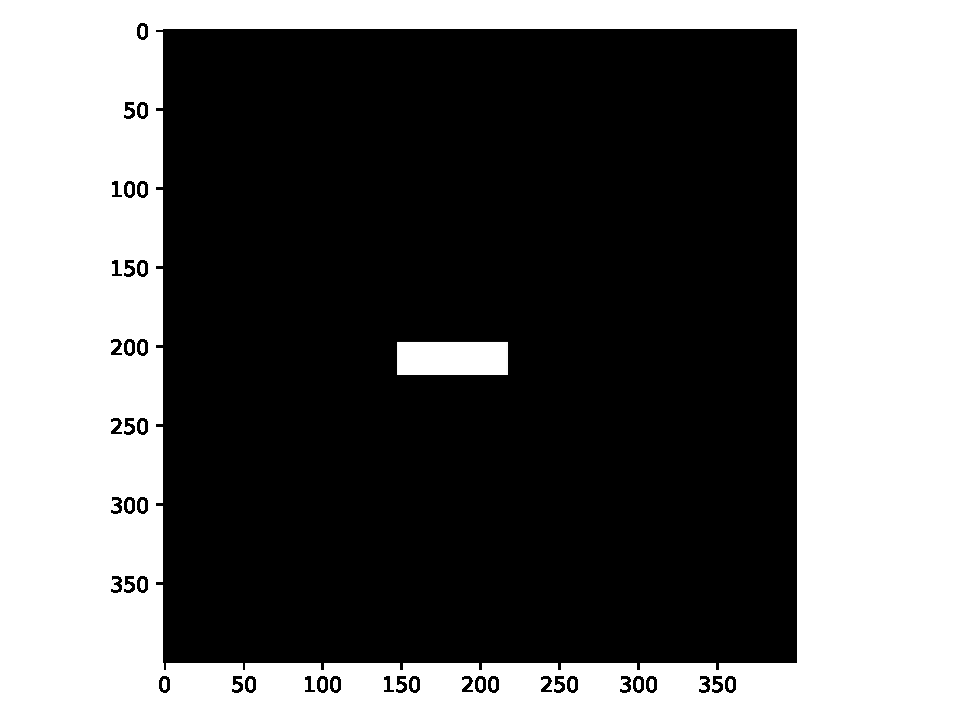
\includegraphics[width=\textwidth]{img/model_demo_2}
            \caption{Ziel}
        \end{subfigure}
    \end{figure}
\end{frame}

\begin{frame}{Modellvorhersage}
    \begin{figure}
        \centering
        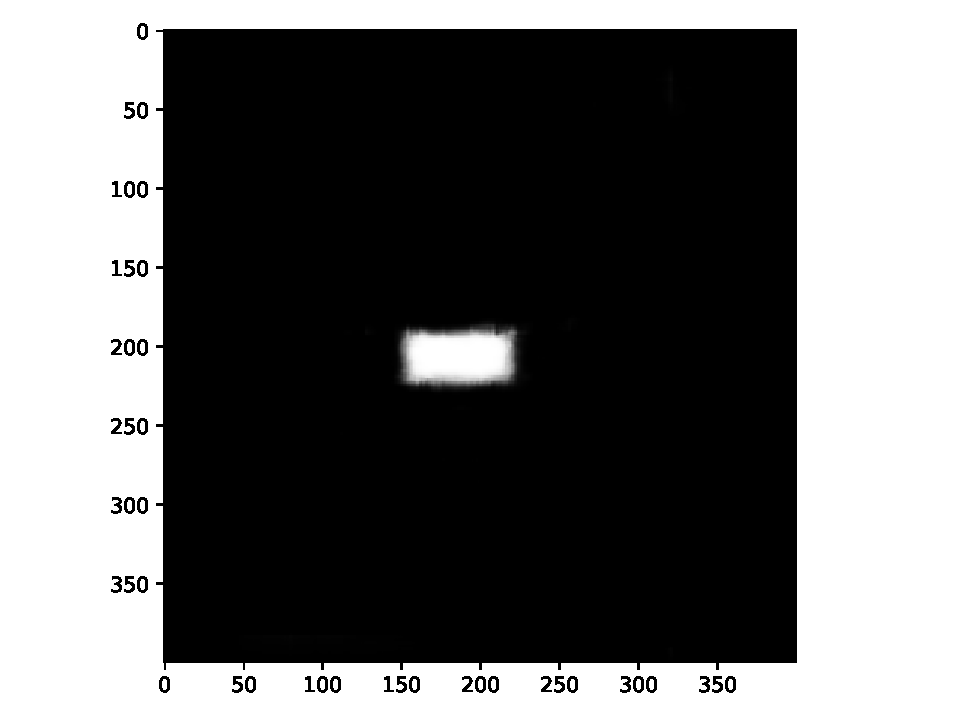
\includegraphics[width=0.9\textwidth]{img/model_demo_3}
    \end{figure}
\end{frame}

\begin{frame}{Schwellenwert}
    \begin{figure}
        \centering
        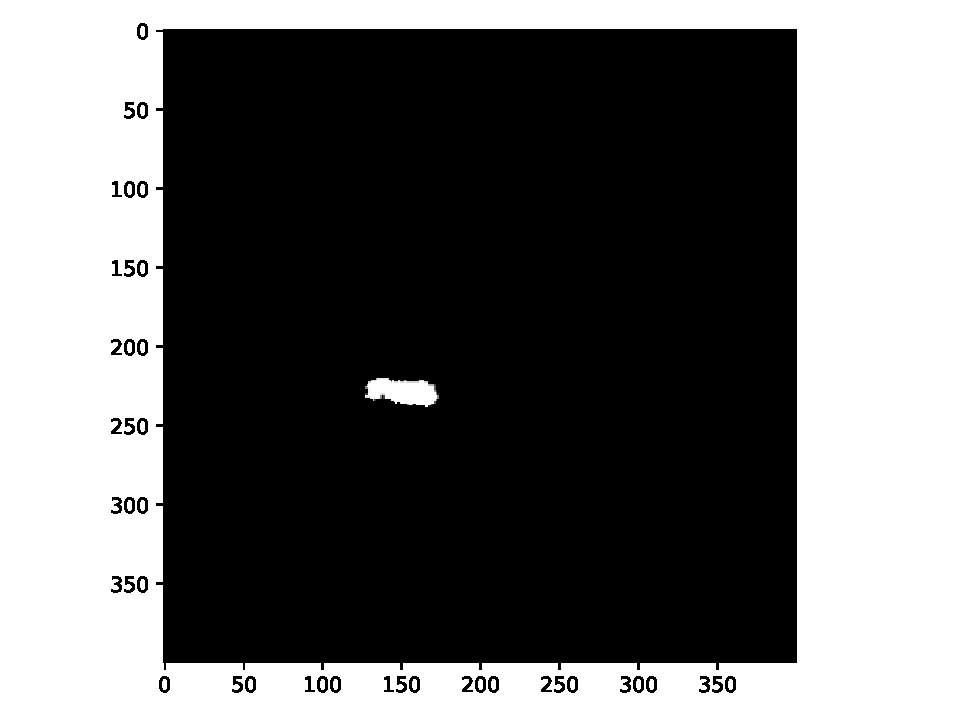
\includegraphics[width=0.9\textwidth]{img/model_demo_4}
    \end{figure}
\end{frame}

\begin{frame}{Umschlie{\ss}endes Rechteck}
    \begin{figure}
        \centering
        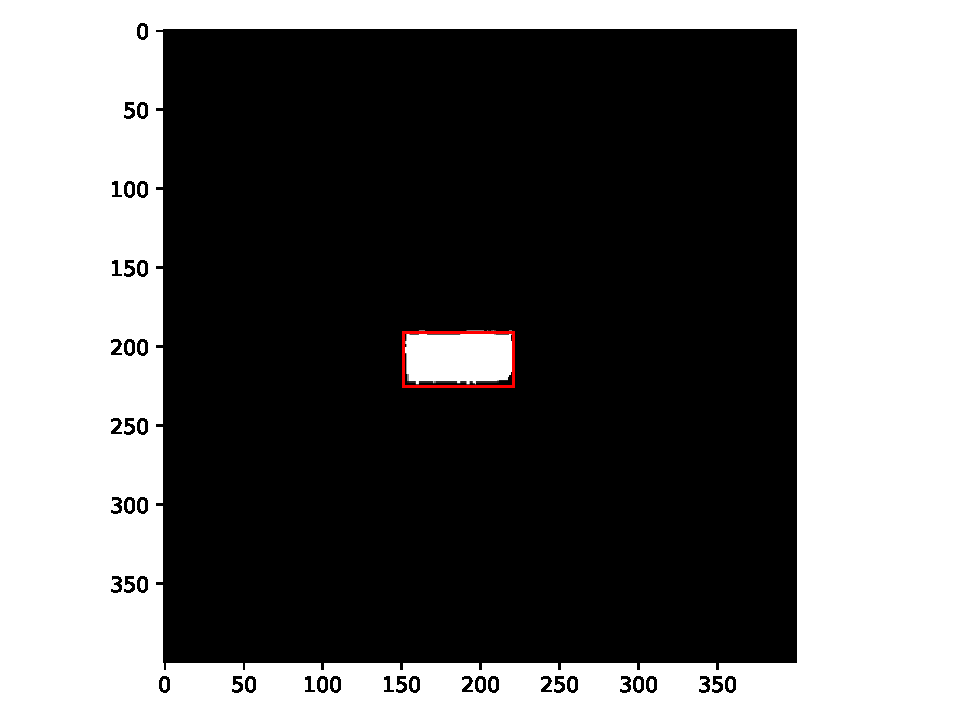
\includegraphics[width=0.9\textwidth]{img/model_demo_5}
    \end{figure}
\end{frame}

\begin{frame}{Resultat}
    \begin{figure}
        \centering
        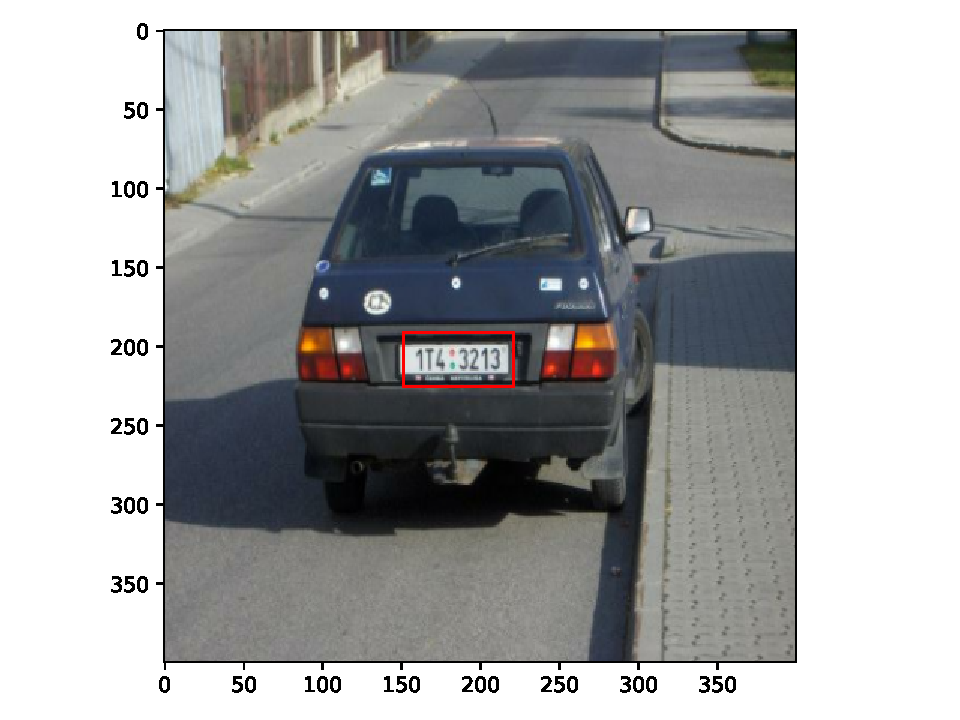
\includegraphics[width=0.9\textwidth]{img/model_demo_6}
    \end{figure}
\end{frame}
